\section{Dérives et Ethique}

\paragraph{Eugénisme, dérives}

\paragraph{} Dans une société où les technologies se multiplient, et où la compétition prend place
à tous les niveaux de nos vies, les spéculations ont commencé à affluer autour d'un terme : l'eugénisme.
Il désigne l'ensemble des recherches (biologiques, génétiques) et des pratiques morales et sociales
ayant pour objectif de \guillemotleft déterminer les conditions les plus favorables à la procréation
de sujets sains et, par là même, d'améliorer la race humaine\guillemotright  \cite{Eugenisme0}. Cette
définition, selon nous, est exactement \emph{la caractérisation de l'application du contrôle} à l'espèce
humaine. Au-delà de l'utilisation du terme de \emph{race humaine} qui nous semble abusive, l'ensemble des
outils de contrôles nécessaires sont réunis : la régulation de la Vie par la génétique et la biologie, la
linéarisation des pensées par la propagande sociale, tout cela derrière une volonté apparente de faire le bien.

\paragraph{Génétique et eugénisme} Sur le point de vue génétique, il existe aujoud'hui plusieurs sociétés
vous proposant de faire analyser votre ADN à partir d'un échantillon de salive. Pour ceux qui hésiteraient,
un marketing travaillé met en avant les avantages du test : connaître ses origines, sa tolérance à divers
aliments.. La société 23andMe met pour cela en scène, à travers de courtes vidéos, l'avis de personnes
ayant tiré une expérience positive du test génétique \cite{23andMe}. Les applications peuvent être 
encore plus poussées, comme chez Pathway Genomics par exemple \cite{Pathway0}. Ici, il s'agit d'un réel
\emph{merchandising} fondé sur l'étude de l'ADN : améliorer sa peau, déterminer sa tolérance au gluten, 
trouver l'équilibre mental..

\paragraph{} La possibilité de dérive sur l'utilisation de ces données nous semble évidente. La définition
que nous avons dressé de la collecte en première partie (voir \ref{collect_data_conscious}) nous fait nous 
demander \emph{la contrepartie} que tirent ces sociétés d'offrir un tel service. Bien entendu, ce dernier 
s'inscrit dans une optique de recherche en génétique, et l'étude des résultats permet certainement une
meilleure compréhension de la population et du génotype humain. Pourtant, bien que les sociétés prétendent
garantir une anonymité totale des données, il nous est compliqué de le conçevoir alors que \emph{la valeur
de la donnée humaine} n'a jamais été \emph{aussi importante}. 

\paragraph{} De plus, au-delà de la question de la \emph{confiance} que nous pouvons placer dans ces entités,
nous ne pouvons passer à côté des applications possibles sur ces données. Que se passerait-il si les hôpitaux
bénéficaient des données génétiques de \emph{chaque patient} ? Si les états décidaient de \emph{réguler la
procréation} pour, sous couvert d'une amélioration de la société, procéder à un \emph{eugénisme intensif} ?
Nous avons vu que les moyens dont nous disposons aujourd'hui, aussi bien en termes de \emph{structures réseaux}
que de \emph{machine learning}, permettraient à une entité de mettre en place ce type de systèmes. Dans un état
totalitaire, comme en Corée du Nord par exemple, le gouvernement pourrait tenter d'établir une population
d'humains augmentés - qui résisteraient mieux aux maladies, qui seraient plus forts, plus intelligents, vivraient
plus longtemps - et ce afin de tenter possèder un avantage stratégique militaire et culturel.

\paragraph{} Même si ces scénarii semblent lointains, nous souhaitons avant tout alerter sur \emph{le fait
qu'il soient réalisables aujourd'hui}. Néanmoins nous pensons que la population - française du moins - n'est
pas prête à la question de l'eugénisme, qui créerait un clivage entre le pour et le contre. Pourtant, rien
n'empêche l'application de \emph{procédés eugéniques} à \emph{des niveaux restreints} de la société. Une
petite partie de la population possède aujourd'hui la majorité des richesses, et les habitudes de vie de
cette partie sont peu connues du reste de la population. La chirurgie esthétique, allégorie simpliste de
\emph{l'augmentation de l'être humain}, n'est réservée qu'à une population possédant \emph{les moyens de se
l'offrir}. Il en sera selon nous de même pour l'eugénisme : seuls ceux en possédant les moyens pourront se
permettre de tenir compte de l'étude d'un ADN. Par ailleurs, et en considérant que l'humanité compte plus
de 8 milliards d'êtres humains (et que ce nombre ne cesse d'augmenter), nous posons la question suivante :
est-il à l'avantage des \emph{classes dirigeantes} de procéder à une \emph{eugénisation générale} de
la société ? Rien n'est moins sûr..

\paragraph{Progrès et dystopies} En ouverture de cette étude fondée sur la génétique, nous souhaitions revenir
un instant sur une grande découverte ayant fait parler d'elle courant 2015 : CRISPR-Cas9. \cite{Genetique0} Ces
\emph{ciseaux génétiques} permettent de \emph{couper une séquence} spécifique d'ADN, afin de la remplacer par
une autre. Cela rend en particulier possible \emph{l'inactivation ou l'activation} de gènes spécifiques.

\begin{figure}[h]
    \centering
    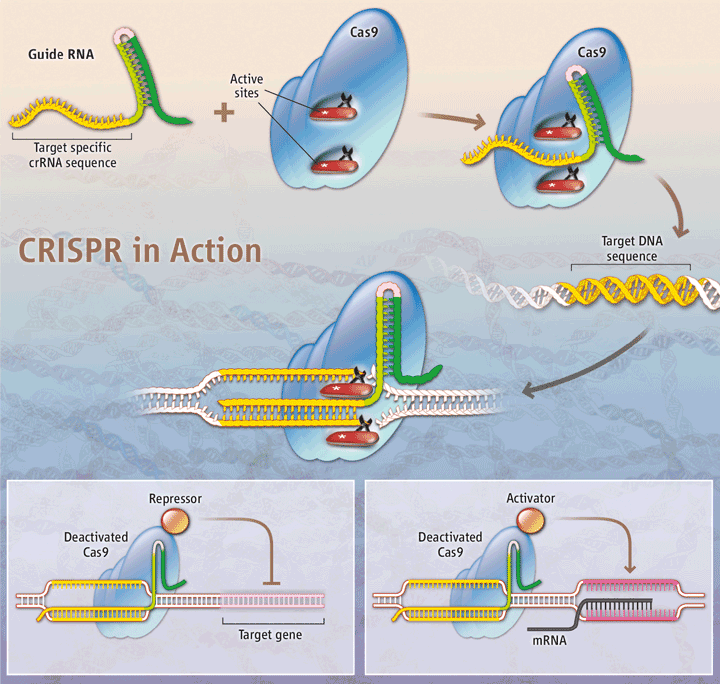
\includegraphics[width=250px]{chapters/03/images/crispr.png}
    \caption{\label{crispr-cas9}\emph{CRISPR-Cas9}, \url{http://www.cite-sciences.fr/fr/ressources/science-actualites/detail/news/crispr-cas9-le-couteau-suisse-qui-revolutionne-la-genetique/}}
\end{figure}

\paragraph{} Couplé à ce que nous venons de voir précédemment sur l'étude du génotype humain, il semble que
l'homme augmenté soit \emph{à portée de main}. Cela nous renvoie à la conférence d'Alain Damasio, \emph{Très humain
plutôt que Transhumain} \cite{Damasio2}, où il statue que l'intégration de la machine à l'homme lui supprime \emph{
sa puissance}. Dans le cas de CRISPR-Cas9 et de la manipulation génétique, il n'est plus question de machines
mais bien de l'Homme lui-même, puisque c'est son \emph{code source} qui est modifié. Peut-on alors, dans ce sens,
statuer que l'amélioration génétique supprime sa puissance à l'Homme ? TODO

\paragraph{Améliorations de vie et sociales}

\paragraph{} Applications \emph{non-intrusives}. Conseil à l'utilisateur plutôt que décision. Exemple médical.
Adaptation au domaine juridique et aux juridictions en proposant des solutions.

\paragraph{} Repartir de la suppression des barrières (langues, traditions etc..). Présenter les SmartCities sous
un jour moins austère à travers la transparence des données de la collectivité mais pas forcément des individus.

\paragraph{} En supprimant les barrières et en recréant un contexte favorable à l'acceptation des différences de tous,
oui. Néanmoins la technologie ne peut pas gommer les divergences d'opinions, en particulier extrémistes, et n'a donc
pas réponse à tout.

\paragraph{} 

** Notre ouverture sur un monde meilleur

\paragraph{Manifeste de l'Ethique Informatique}

\begin{itemize}
    \item Notre priorité absolue est l'établissement d'une
    meilleure symbiose entre la technologie et le genre humain.

    \item L'objectif de toute production logicielle doit être
    l'éducation de l'humanité par le développement
    d'applications intuitives, non-invasives et évolutives.

    \item L'utilisateur doit toujours être en contrôle de la
    récolte et de l'utilisation de ses données personnelles.

    \item L'ensemble des projets informatiques ayant un impact
    sur l'humain doivent être consultables librement.

    \item La donnée, à l'image de l'Homme, ne se concrétise qu'en
    réseaux. C'est pourquoi ces derniers doivent demeurer incontrôlés 
    par toute minorité.

    \item L'Intelligence Artificielle doit accompagner l'Homme pour
    lui permettre d'exprimer sa puissance sans la déléguer
    à la machine.

    \item Les technologies ne doivent d'aucune manière permettre de 
    sélectionner ou de distinguer les Hommes.
\end{itemize}

\paragraph{} L'éducation par l'expérience de la Nature doit
demeurer notre première orientation.
